\documentclass[letterpaper,12pt,spanish]{article}
\usepackage{amssymb}
\usepackage{amsmath}
\usepackage{amsfonts}
\usepackage{graphicx}
\usepackage{babel}
\usepackage[utf8]{inputenc}
\usepackage{hyperref}
\usepackage{fleqn}
\usepackage{fancyhdr}
\usepackage{multirow}
\usepackage{multicol} 
\usepackage{anysize}
\pagestyle{fancy}

\marginsize{2,5cm}{2,5cm}{0,5cm}{1,8cm}

\pagestyle{fancy}


\hypersetup{pdfpagemode=UseOutlines}
\hypersetup{colorlinks=true}
\hypersetup{urlcolor=red}
\hypersetup{linkcolor=blue}
\hypersetup{citecolor=black}

\fancyfoot{}
\fancyhead[LE,RO]{
\includegraphics[scale=0.82]{imagenes/logoinf.jpg}}
\fancyhead[LO,RE]{
\includegraphics[scale=0.3]{imagenes/logo_usm.JPG}}
\fancyfoot[LE,RO]{\thepage}
\fancyfoot[LO,RE]{Taller de Herramientas Modelado de Procesos de Negocio}
\renewcommand{\headrulewidth}{0.4pt}
\renewcommand{\footrulewidth}{0.4pt}

\renewcommand{\sfdefault}{phv} 
%\sffamily %trabaja con helvetica en el cuerpo del documento
%\renewcommand{\rmfamily}{phv} % permite trabajar con helvetica los títulos

%\renewcommand{\familydefault}{phv} % permite trabajar con letra helvetica los títulos


\author{
{\normalsize Patricia Fredes Arce 2584080-1}\\
{\normalsize Maria José Polloni Fuentes 2873042-k}\\
{\normalsize Margarita Ortega Rodriguez 2773024-8}\\
{\normalsize Fernando Morales 2573034-8}\\
}
\title{\vspace{-1cm}
\includegraphics[scale=0.5]{imagenes/logo_usm.JPG}\\\vspace{-0.2cm}
    {\small \scshape Universidad T\'ecnica Federico Santa Mar\'ia}\\
    \vspace{1cm}
    {\bfseries Taller de Herramientas de Modelado de Procesos de Negocio} \\ {\Large Proyecto 1: Etapa 1} \\\vspace{0.2cm}{\normalsize Viktor Tapia}
}
\date{Valpara\'iso, 5 de Octubre del 2012.}

\begin{document}
\maketitle
\thispagestyle{empty}
\newpage
\tableofcontents
\newpage

\section{Introducción}
En este informe se realiza el modelado de los procesos de negocio de la panadería Rodenas que está ubicada en Rancagua, donde fabrica, vende y distribuye sus productos a lo largo de gran parte de la provincia del Cachapoal. Nace 1948 aproximadamente, en la localidad de Coya desde donde se expande hacia la ciudad de Rancagua, por la iniciativa e involucramiento de los hijos del fundador. En este momento va en la tercera generación de gestión, teniendo 20 trabajadores repartidos en distintos turnos, y otras panaderias con el mismo nombre pero sin relacion comercial con la panaderia en estudio, los lazos son meramente familiares.
Como misión manifiesta la de producir y vender pan de buena sabor, aspecto y duradero en el tiempo. Entregando productos de calidad en la región manteniendo la costumbre chilena en la fabricación de este.
La filosofía de la empresa con respecto a sus proyecciones o visión es bastante limitada. Manteniendo la postura de “vivir el día a día”, acortando la mirada a plazos lo más pequeño posible posible. De esta manera se ha mantenido más de 60 años funcionando, con todos los altos y bajos que ha manifestado la industria.
\\
Para efectos de este proyecto, se ha incorporado la sección ``reposteria", la cual se encarga de producir tortas, pasteles y galletas. Cabe destacar que son procesos extraidos de la panadería del supermercado Hiper Lider 15 norte de la ciudad de Viña del mar. Si bien, la diferencia en cuanto a tamaño de ambos, es grande, el proceso que se debe hacer para su producción es el mismo. \\
Además es posible que este mecanismo tambien ayude a la empresa de panadería ampliar sus rangos de venta hacia la repostería.

\section{Herramienta}
La herramienta que se utilizará para realizar el modelo de los procesos de negocios de la panadería Rodenas es el software \textbf{"Bizagi Process Modeler"}.

%\newpage
\section{Criterios a evaluar y analisis}
Los criterios a evaluar fueron estimados con el rango de notas de 1 a 7, sacando un promedio de cada integrante del equipo según la percepción que obtuvo al utilizar el software: \\

\begin{center}
\begin{tabular}{|l|c|p{2.40in}|}
 \hline
 \textbf{Criterio} & \textbf{Nota} & \textbf{Comentario} \\
 \hline
 \textbf{Fácil de Implementar} & 7.0 & Es una herramienta 100\% web, por lo que no necesariamente el software necesita ser instalado en el computador. \\
 \hline
 \textbf{Facilidad de uso} & 5.0 & Presenta una interfaz poco intuitiva (Diseño Drag and Drop). \\
 \hline
 \textbf{Estándares} & 6.0 & No utiliza la misma notación de BPMN 2.0 pero son semejantes, su notación esta orientada a SOA (arquitectura orientada a servicios). \\
 \hline
 \textbf{Licencia} & 7.0 & ProcessMaker brinda a las organizaciones las ventajas de open source. \\
 \hline
 \textbf{Documentación y Soporte} & 7.0 & La página web del software presenta una gran variedad de documentación , vídeos y foros en que se enseña a utilizar el software, además posee un servicio de soporte. \\
 \hline
\end{tabular}
\end{center}

\subsection{Ejemplo de Proceso de obtención de tarjeta de crédito}
Para la utilización del software ProcessMaker, según el modelamiento de procesos, se utilizó como referencia un video de youtube que explicaba la obtención de una tarjeta de crédito en un banco.

También se pudo observar que este software posee la capacidad de que el administrador pueda interactuar con cualquier trabajador de la empresa en algún proceso, puesto que existe la opción de agregar usuarios, grupos o departamentos, en que el administrador puede asignarles tareas o sub-tareas, también poder enviarles reportes, mensajes (en el mismo software hay un inbox) o mails. Además esta la opción que si alguna tarea requiere de la creación de formularios, se realiza de forma dinámica, en el ejemplo de la tarjeta de crédito se requiere en la tarea de ``Rellenar Solicitud", un formulario en que se ingresen los datos del cliente y fecha en que se realizó la solicitud, entonces en esta tarea el usuario de la empresa asignado en esta tarea tendrá la misión de ingresar mediante este formulario los clientes que serán luego guardados en una base de datos del mismo software.
 
\begin{center}
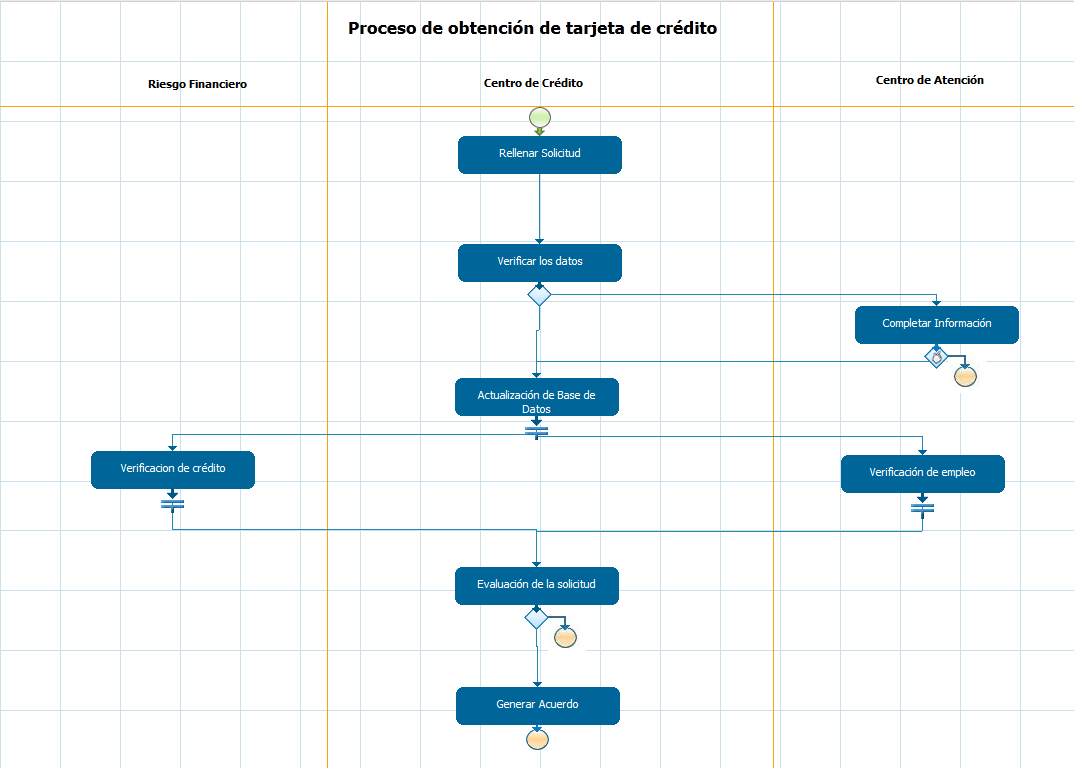
\includegraphics[scale=0.5]{./imagenes/modelos_pm.png}\\
     Figura 1: Modelo en Process Maker.\\
\end{center}

A continuación se muestra la notación del software:

%ingresar la notación

\section{Criterios a evaluar}
\input{./src/ejemplo_proceso.tex}

\section{Conclusiones}
En cuanto a las conclusiones podemos decir, que modelar los procesos de una panadería es especialmente ideal, puesto que posee claramente identificados los roles de cada participante de las actividades que se deben realizar.\\
Se observa que la mayor parte de los procesos tienen como responsable al administrador de la organización, por lo que como mejora, si es que la carga es muy grande, se podría delegar esta responsabilidad a otra persona siendo el administrador solo supervisor de los procesos.\\
Por otro lado, como lo describimos al comienzo, si se realizan los cambios y extensiones pertinentes, es posible ampliar el rango de ventas de la panaderia, añadiendo una sección repostería que permitiera vender tortas, galletas y/o pasteles.\\
En cuanto a la herramienta utilizada, es bastante fácil de utilizar, pues contiene todos los elementos de la notación BPMN 2.0 y está especialmente diseñado para este fin, en contraste con la herramienta ProcessMaker, la cual es un poco menos intuitiva además de no incorporar todos los elementos necesarios para el modelamiento, pero si para gestionarlos.

\bibliographystyle{alpha}
\bibliography{bibbase}
 
\end{document}